\documentclass[10pt, a4paper]{amsart}
% \documentclass[10pt,showpacs,preprintnumbers,footinbib,amsmath,amssymb,aps,prl,twocolumn,groupedaddress,superscriptaddress,showkeys]{revtex4-1}
\usepackage[]{graphicx}
\usepackage[]{hyperref}
\usepackage[]{physics}
\usepackage[]{listings}
\usepackage[T1]{fontenc}
\usepackage{color}
\usepackage[]{subcaption}
\usepackage[ruled,vlined]{algorithm2e}

\definecolor{mygreen}{rgb}{0,0.6,0}
\definecolor{mymauve}{rgb}{0.58,0,0.82}

\lstset{ %
  backgroundcolor=\color{white},   % choose the background color; you must add \usepackage{color} or \usepackage{xcolor}
  basicstyle=\footnotesize,        % the size of the fonts that are used for the code
  breakatwhitespace=false,         % sets if automatic breaks should only happen at whitespace
  breaklines=true,                 % sets automatic line breaking
  captionpos=b,                    % sets the caption-position to bottom
  commentstyle=\color{mygreen},    % comment style
  deletekeywords={...},            % if you want to delete keywords from the given language
  escapeinside={\%*}{*)},          % if you want to add LaTeX within your code
  extendedchars=true,              % lets you use non-ASCII characters; for 8-bits encodings only, does not work with UTF-8
  frame=single,	                   % adds a frame around the code
  keepspaces=true,                 % keeps spaces in text, useful for keeping indentation of code (possibly needs columns=flexible)
  keywordstyle=\color{blue},       % keyword style
  language=c++,                    % the language of the code
  otherkeywords={*,...},           % if you want to add more keywords to the set
  rulecolor=\color{black},         % if not set, the frame-color may be changed on line-breaks within not-black text (e.g. comments (green here))
  showspaces=false,                % show spaces everywhere adding particular underscores; it overrides 'showstringspaces'
  showstringspaces=false,          % underline spaces within strings only
  showtabs=false,                  % show tabs within strings adding particular underscores
  stepnumber=2,                    % the step between two line-numbers. If it's 1, each line will be numbered
  stringstyle=\color{mymauve},     % string literal style
  tabsize=2,	                     % sets default tabsize to 2 spaces
}


\title[Solving the Poisson-equation in one dimension]{Solving the Poisson-equation in one dimension: \\
\normalsize{Tridiagonal Matrix Algorithm\\
 and \\
 LU-decomposition} \\
  \hrulefill\small{ FYS3150: Computational Physics }\hrulefill}

\author[Sundberg]{Sigurd Sandvoll Sundberg \\
  \href{https://github.com/SigurdSundberg/FYS3150/tree/master/project1}{\texttt{github.com/sigurdsundberg}}}

\begin{document}

\begin{titlepage}
\begin{abstract}
The one-dimensional Poisson equation has been solved by developing two versions tridiagonal matrix algorithm, including using known methods of solving linear equations, in LU decomposition and Armadillos $solve()$. We look at the numerical accuracy, run time and memory used by the different algorithms. Our tridiagonal matrix algorithms, are found to be considerably faster than LU decomposition, with a factor of ~1000. As well as needing a lot less memory. For solving numerical problems it is important to develop algorithms to solve our problems efficiently where possible. This is to reduce loss of numerical precision, memory needed and run time. We found that for our general algorithm, the optimal steplength was $\sim10^{5}$, whilst for our specialized algorithm the steplength was $\sim10^{6}$. 
\end{abstract}
\maketitle
\tableofcontents
\end{titlepage}

\section{Introduction}
Linear second-order differential equations plays a central part in science and solving these numerically save us many many hours of struggeling to find analytical solutions to these equations. The differential equations can be manipulated to linear algebra problems, for which we can develop algorithms to solve to problems numerically. There are limitations when it comes to numerically solutions. If the number of floating point operations(FLOPs) becomes too big the calculations can get exceedingly slow. Another risk is loss of numerical precision from how numbers are stored in a computer and the amount of FLOPs we perform. This puts the emphasis on developing algorithms which are stable, accurate and quick. 
In this project we will take a look at solving the one-dimensional Poisson equation with Dirichlet boundary conditions by rewriting it as a set of linear equations. Excplicitly we want to solve the following equation
\begin{equation}
-u''(x) = f(x), \quad x\in(0,1), \quad u(0)=u(1)=0.\label{eq:base}
\end{equation}
Firstly the background for the Poisson equations, how the second derivative can be approximated and theory behind LU decomposition will be presented. Secondly, two algorithms will be developed and implemented through psuedocode. Thirdly, the performance of the algorithms will be presented. Lastly, the findings will be discussed and some concluding remarks. 


\section{Theory}
\subsection{Poisson equation}
A classic exmaple of linear second-order differential equation is the Poisson's equation from electromagnetism. The electrostatic potential $\Phi$ is generated by localized charge distribution $\rho(\mathbf{r}.$ The equation read 
\begin{equation}
	\nabla^2\Phi = -4\pi\rho(\mathbf{r})\nonumber.
\end{equation}
If we have spherical symmetric $\Phi$ and $\rho(\mathbf{r}$ the equations simplifies to one-dimensional equation in $r$, namely 
\begin{equation}
	\frac{1}{r^2}\frac{d}{dr}\left( r^2\frac{d\Phi}{dr}\right) = -4\pi\rho(r).	\nonumber
\end{equation}
By substituting $\Phi(r) = \phi(r)/r$ we get 
\begin{equation}
	\frac{d^2\phi}{dr^2} = -4\pi r\rho(r).\nonumber
\end{equation}
This is a linear second-order differential equation on the form in equation \ref{eq:base} with $\phi \rightarrow u$, $r \rightarrow x$ and $f(x) = 4\pi r\rho(r)$. We are left with
\begin{equation}
	-u''(x) = f(x)\nonumber
\end{equation}

In our study the source term will be $f(x) = 100e^{-10x}$ and and the analytical solution is given by $u(x) = 1-(1-e^{-10})x-e^{-10x}$, this can be verified easily by taking the second derivative of $u(x)$.
\subsection{Approximating the second derivative}
% >> Going from diff to linear form 
To solve one-dimensional Poisson equiation numerically we will need to discretize the equation. Instead of having continous functions, we get 
\begin{equation}\label{eq:disc}
	\begin{split}
		x \rightarrow x_i\in[x_0,x_1, \dots ,x_i,\dots ,x_{n+1}]\\
		u(x) \rightarrow u(x_i) = u_i \in[u_0,u_1, \dots ,u_i,\dots ,u_{n+1}]\\	
		f(x) \rightarrow f(x_i) = f_i \in[f_0,f_1, \dots ,f_i,\dots ,f_{n+1}],
	\end{split}
\end{equation}
using grid-points $x_i = ih$ in the interval from $x_0 = 0$ to $x_{n+1} = 1$ since we have an open interval. The step length h is defined as $h = 1/(n+1)$. We then have the boundary conditions $x_0 = v_{n+1} = 0$. The approximation for the second derivative we need from \ref{eq:base}, can be found through Taylor expansion of $u(x\pm h)$ around $x$.
\begin{equation}
	u(x\pm h) = u(x) \pm hu'(x) + \frac{h^2u''(x)}{2!} \pm \frac{h^3u'''(x)}{3!} + \mathcal{O}(h^4)\label{eq:taylor_exp}
\end{equation}
If we look at the two equation we get from $u(x+h)$ and $u(x-h)$, we can see that the first and third derivatives cancel eachother out when we add the two equations together. If we solve the resulting equation for $u''(x)$ we get 
\begin{equation}
u''(x) = \frac{u(x+h) + u(x-h) - 2u(x)}{h^2} + \mathcal{O}(h^2).\label{eq:second_der}
\end{equation}
Using our discretization of the continous functions given by equation \ref{eq:disc}, we have the following equation
\begin{equation}
-u''(x) \simeq f_i = \frac{u_{i+1} + u_{i-1} -2u_i}{h^2} +\mathcal{O}(h^2). \label{eq:inserted_for_disc}
\end{equation}
for $i = 1,\cdots , n$. 
If we define $f^*_i = h^2f_i$, equation \ref{eq:inserted_for_disc} becomes $-u_{i+1} - u_{i-1} +2u_i = f^*_i$. If we try inserting values of $i= 1, 2, 3, 4,\dots , n-1 n$  we get the following
\begin{equation}\label{eq:disc_ins_i}
	\begin{split}
		-u_2 - u_0 + 2u_1 = f^*_1 \quad i = 1\\
		-u_3 - u_1 + 2u_2 = f^*_2 \quad i = 2\\
		-u_4 - u_2 + 2u_3 = f^*_3 \quad i = 3\\
		-u_5 - u_3 + 2u_4 = f^*_4 \quad i = 4\\
		\vdots \\
		-u_n - u_{n-2} + 2u_{n-1} = f^*_{n-1} \quad i = n-1\\
		-u_{n+1} - u_{n-1} + 2u_n = f^*_n \quad i = n
	\end{split}
\end{equation}
With the Dirichlet boundary conditions $u(0) = u(n+1) = 0$ we see resembles a matrix with $2$ along the diagonal and $-1$ directly above and below the leading diagonal. We see that we can solve as a linear algebra problem, where we want to find $\vec{x}$, on the following form. 
\begin{equation}
\mathbf{A}\vec{x} = f^*, \nonumber
\end{equation}
where $\mathbf{A}$ is an $n\times n$ tridiagonal matrix which we found in \ref{eq:disc_ins_i}.
\begin{equation}\label{mat:tridiag_1_n}
\mathbf{A} = 
\begin{bmatrix}
2 & -1 & 0 & \dots & \dots & 0 \\
-1 & 2 & -1 & 0 & \dots & \dots \\
0 & -1 & 2 & -1 & 0 & \dots \\
\dots & \dots & \ddots & \ddots & \ddots & \dots\\
0 & \dots & 0 & -1 & 2 & -1 \\
0 & \dots & \dots & 0 & -1 & 2
\end{bmatrix}
\end{equation}

\subsection{LU decomposition}
The general method for solving linear equations with dense non-singular matricies is using LU decomposition. The method involves taking a matrix $\mathbf{A}$ and rewriting it into the product of a lower triangular matrix $\mathbf{L}$ and an upper triangular matrix $\mathbf{U}$. 
\begin{align*}
\mathbf{A} &= \mathbf{L}\mathbf{U}\\
\begin{bmatrix}
	a_{11} & a_{12} & a_{13} & a_{14} \\
	a_{21} &a_{22} &a_{23} &a_{24} \\
	a_{31} &a_{32} &a_{33} &a_{34}  \\
	a_{41} &a_{32} &a_{43} &a_{44} 
\end{bmatrix}
&= 
\begin{bmatrix}
1& 0 & 0 & 0 \\
 l_{21}& 1& 0 & 0\\
 l_{31}&l_{32}&1& 0\\
 l_{41}&l_{42}&l_{43}&1
\end{bmatrix}
\begin{bmatrix}
u_{11}& u_{21}&u_{31}&u_{41}\\
0 & u_{22} & u_{23}& u_{24} \\
0 & 0 & u_{33}& u_{34}\\
0 & 0 & 0 & u_{44}
\end{bmatrix}
\end{align*}

This gives us a new way of solving $\mathbf{A}\vec{x}=\vec{b}$, where we can look at simpler equations to solve the problem
\begin{equation}
\mathbf{L}\mathbf{U}\vec{x} = \vec{b} \rightarrow \mathbf{L}\vec{w} = \vec{b}, \quad \mathbf{U}\vec{x} = \vec{w}
\end{equation}
Where the above set of equations can be solved through backwards substitution. 

\section{Algorithms} 
For all programs, benchmark calulations and plots, see: \\
\href{https://github.com/SigurdSundberg/FYS3150/tree/master/project1}{\textbf{github.com/SigurdSundberg/FYS3150}}


\subsection{Tridiagonal Matrix Algorithm}
Looking at a general case of solving a tridiagonal matrix on the form $\mathbf{A}\vec{x} = f^*$ we have 
\begin{equation} 
	\begin{bmatrix}
		b_1 & c_1 & 0 &\dots &\dots &\dots \\
		a_1 & b_2 & c_2 & 0 &\dots &\dots\\
		0 & a_2 & b_3 & c_3 & 0 &\dots \\
		\dots &\dots &\dots &\dots &\dots &\dots\\
		\dots &\dots &\dots & a_{n-2} & b_{n-1} & c_{n-1} \\
		\dots &\dots &\dots &\dots &a_{n-1} & b_n
	\end{bmatrix}
	\begin{bmatrix}
		x_1 \\
		x_2 \\
		\dots \\
		\dots \\
		\dots \\
		x_n
	\end{bmatrix} 
	= 
	\begin{bmatrix}
		f^*_1\\
		f^*_2\\
		\dots \\
		\dots \\
		\dots \\
		f^*_n
	\end{bmatrix}
\end{equation}

Let's take general case for a $4\times 4$ tridiagonal matrix and use Gaussian elimination to see if we can spot a pattern.
Our system can then be written 
\begin{align}
	\mathbf{A}\vec{x} &= f^*\nonumber\\
	\begin{bmatrix}
		b_1 & c_1 & 0 & 0\\
		a_1 & b_2 & c_2 & 0\\
		0 & a_2 & b_3 & c_3 \\
		0 & 0 & a_3 & b_4 
	\end{bmatrix}
	\begin{bmatrix}
		x_1\\
		x_2\\
		x_3\\
		x_4
	\end{bmatrix}
	&= 
	\begin{bmatrix}
		f^*_1\\
		f^*_2\\
		f^*_3\\
		f^*_4
	\end{bmatrix}
\end{align}

The set of equations we will use Gaussian elimination on is therefore 
\begin{equation}
 \left[
  \begin{array}{cccc|c}
	b_1 & c_1 & 0 & 0 & f^*_1\\
	a_1 & b_2 & c_2 & 0 & f^*_2\\
	0 & a_2 & b_3 & c_3 & f^*_3\\
	0 & 0 & a_3 & b_4 & f^*_4
  \end{array}
 \right]
\end{equation}
First we will use forward substitution to remove all the elements along the diagonal below the leading diagonal. We start with $\textrm{II} - \textrm{I}(a_1/b_1)$ to remove $a_1$ from $\textrm{II}$, where \textrm{I} refers to row one, \textrm{II} refers to row two and so on. We now how 
\begin{equation}
	\left[
  \begin{array}{cccc|c}
	b_1 & c_1 & 0 & 0 & f^*_1\\
	0 & b_2- c_1a_1/b_1 & c_2 & 0 & f^*_2 - f^*_1a_1/b_1\\
	0 & a_2 & b_3 & c_3 & f^*_3\\
	0 & 0 & a_3 & b_4 & f^*_4
  \end{array}
 \right]
\end{equation}
We will define two new variables $\tilde{b}_2 =b_2- c_1a_1/b_1 $ and $\tilde{f}_2 = f^*_2 - f^*_1a_1/b_1$ to simplify the matrix and continue the forward substitution with $\textrm{III} - \textrm{II}(a_2/\tilde{b}_2)$.
\begin{equation}
 \left[
  \begin{array}{cccc|c}
	b_1 & c_1 & 0 & 0 & f^*_1\\
	0 & \tilde{b}_2 & c_2 & 0 & \tilde{f}_2\\
	0 & 0 & b_3-c_2a_2/\tilde{b}_2 & c_3 & f^*_3-\tilde{f}_2a_2/\tilde{b}_2\\
	0 & 0 & a_3 & b_4 & f^*_4
  \end{array}
 \right]
\end{equation}
Using the same definition as above as prior $\tilde{b}_i = b_i -c_{i-1}a_{i-1}/b_{i-1}$ and $\tilde{f}_i = f_i - f_{i-1}a_{i-1}/b_{i-1}$ we are left with 
\begin{equation}
\left[
  \begin{array}{cccc|c}
	b_1 & c_1 & 0 & 0 & f^*_1\\
	0 & \tilde{b}_2 & c_2 & 0 & \tilde{f}_2\\
	0 & 0 & \tilde{b}_3 & c_3 & \tilde{f}_3\\
	0 & 0 & a_3 & b_4 & f^*_4
  \end{array}
 \right]
\end{equation}
Repeating this one more time we can eliminate $a_3$. We see however that we see that a pattern emerges for the forward substitution namely 
\begin{equation}\label{algo:forward_sub}
\begin{split}
	\tilde{b}_i = b_i -\frac{c_{i-1}a_{i-1}}{\tilde{b}_{i-1}} \\
	\tilde{f}_i = f^*_i - \frac{\tilde{f}_{i-1}a_{i-1}}{\tilde{b}_{i-1}}.
\end{split}
\end{equation}
If we define $\tilde{b}_1 = b_1$ and $\tilde{f}_1 = f_1$ and get the follwing matrix 
\begin{equation}
\left[
  \begin{array}{cccc|c}
	\tilde{b}_1 & c_1 & 0 & 0 & \tilde{f}_1\\
	0 & \tilde{b}_2 & c_2 & 0 & \tilde{f}_2\\
	0 & 0 & \tilde{b}_3 & c_3 & \tilde{f}_3\\
	0 & 0 & 0 & \tilde{b}_4 & \tilde{f}_4
  \end{array}
 \right]
\end{equation}
We can now solve for $\vec{x}$ by doing a backwards substitution. We find $x_4$ by doing $\tilde{f}_4/\tilde{b}_4$, giving us 
\begin{equation}\label{sub:back}
\left[
  \begin{array}{cccc|c}
	\tilde{b}_1 & c_1 & 0 & 0 & \tilde{f}_1\\
	0 & \tilde{b}_2 & c_2 & 0 & \tilde{f}_2\\
	0 & 0 & \tilde{b}_3 & c_3 & \tilde{f}_3\\
	0 & 0 & 0 & 1 & x_4
  \end{array}
 \right]
\end{equation}
Doing a backwards substitution on matrix \ref{sub:back} by taking $\textrm{III} - \textrm{IV}(c_3)$ and dividing \textrm{III} by $\tilde{b}_3$ to normalize the row. We then define $x_3 = (\tilde{f}_3 - x_4c_3)/\tilde{b}_3$, which gives us 
\begin{equation}
\left[
  \begin{array}{cccc|c}
	\tilde{b}_1 & c_1 & 0 & 0 & \tilde{f}_1\\
	0 & \tilde{b}_2 & c_2 & 0 & \tilde{f}_2\\
	0 & 0 & 1 & 0 & x_3\\
	0 & 0 & 0 & 1 & x_4
  \end{array}
 \right]
\end{equation}
Repeating the process on row \textrm{II} and using the same definition as above we get
\begin{equation}
\left[
  \begin{array}{cccc|c}
	\tilde{b}_1 & c_1 & 0 & 0 & \tilde{f}_1\\
	0 & 1 & 0 & 0 & x_2\\
	0 & 0 & 1 & 0 & x_3\\
	0 & 0 & 0 & 1 & x_4
  \end{array}
 \right]
\end{equation}
we see that a pattern emerges, namely
\begin{equation}\label{algo:backwards_sub}
	x_i = \frac{\tilde{f}_i - x_{i+1}c_i}{\tilde{b}_i}
\end{equation}
which we will call backwards substitution from now. 

Assuming we have pre initialized vectors $a, b, c, f^*$ and defining $\tilde{b}_1 = b_1$ and $\tilde{f}_1 = 1$, our general algorithm from respectivly \ref{algo:forward_sub} and \ref{algo:backwards_sub} will read as follows
\begin{algorithm}[H]\label{psudo:for}
\SetAlgoLined
 initialization\;
 \For{i = 2, 3, \dots , n}{
  $quotient = a_{i-1}/\tilde{•}tilde{b}_{i-1}$\;
  $\tilde{b}_i = b_i - c_{i-1}\cdot quotient$\;
  $\tilde{f}_i = f^*_i - \tilde{f}_{i-1}\cdot quotient$\;  
 }
\caption{Forward substitution}
\end{algorithm}
\begin{algorithm}[H]\label{psudo:back}
\SetAlgoLined
 $x_n = \tilde{f}_n/\tilde{b}_n$\;
 \For{i = n-1, n-2,\dots , 1}{
	$x_i = (\tilde{f}_i - x_{i+1}c_i)/\tilde{b}_i$\;  
 }
\caption{Backward substitution}
\end{algorithm}

We are also interested in the number of FLOPs for our general algorithm. From the algorithm \ref{psudo:for} we see that for each iteration $i$ of the loop we have 5 FLOPs and in algorithm \ref{psudo:back} we have 3 FLOPs for each iteration $i$ of the loop. Each loop does $n-1$ iterations, thus we have in total $(8(n-1) + 1)$ FLOPs, the $+1$ comes from the initial calculation in algortihm \ref{psudo:back}. So we have in total $8n-7$ FLOPs, for large $n$ we can ignore the cosntant terms and we are left with $8n$ FLOPs for the general algorithm. 
For very large $n$ this will come out to be $\mathcal{O}(n)$, however for comparison purposes we will use $8n$ FLOPs for the general algorithm. 

\subsection{Specialized algorithm}
In our study we have matrix on the form seen in matrix \ref{mat:tridiag_1_n} which as $2$ along the leading diagonal and $-1$ along two other diagonals. Since we have a symmetrical matrix we make it more efficient at solving the problems. If we look at our algortihms \ref{algo:forward_sub} and \ref{algo:backwards_sub} we can insert $b_i = 2$ and $a_i = c_i = -1$ for all $i$ and we get the following expressions
\begin{align}
	\tilde{b}_i &= 2 - \frac{1}{\tilde{b}_{i-1}}\label{spec:pre}\\
	\tilde{f}_i &= f^*_i + \frac{\tilde{f}_{i-1}}{\tilde{b}_{i-1}}\\
	x_i &= \frac{\tilde{f}_i + x_{i+1}}{\tilde{b}_i}
\end{align}
If we take a look at equation \ref{spec:pre}, we can show that the expressions can be rewritten on the form 
\begin{equation}
 \tilde{b}_i \equiv d_i = \frac{i+1}{i}.
\end{equation}
We see this from inserting $i = 2, 3, 4, \dots$. If we take a look at it we get 
\begin{align*}
	d_1 &= 2 \\
	d_2 &= 2 - \frac{1}{2} = \frac{3}{2}\\
	d_3 &= 2 - \frac{1}{\frac{3}{2}} = \frac{4}{3}\\
	d_4 &= 2 - \frac{1}{\frac{4}{3}} = \frac{5}{4}\\
	\vdots\\
	d_i &= \frac{i+1}{i}
\end{align*}
this can be shown to be true through, for example induction. This can be found before our algorithm reducing the number of FLOPs needed in our loops. Psuedocode for our specialized algorithm will be as follows 

\begin{algorithm}[H]\label{psudo:spec}
\SetAlgoLined
 initialization\;
 \For{i = 2, 3,\dots , n}{
	$\tilde{f}_i = f^*_i + \tilde{f}_{i-1}/d_{i-1}$\;  
 }
 $x_n = \tilde{f}_n/d_n$\;
 \For{i = n-1, n-2, \dots, 1}{
	$x_i = (\tilde{f}_i + x_{i+1})/d_i$
 }
\caption{Specialized algortihm}
\end{algorithm}

If we take a look at the number of FLOPs in our specialized algorithm we see that we have 2 FLOPs for each of the loops, running $n-1$ times. Thus our specialized algorithm has in total $4(n-1)+1$ FLOPs $=(4n-3)$ FLOPs. For large $n$ we have $4n$ FLOPs. If we compared this to the generalized algorithm, we see that it is a factor $2$. 

\subsection{LU Decomposition and Armadillo $solve()$}
We will not be developing and implementing an algortihm for LU decomposition. However two different approaches will be used. The high level C++ library Armadillo contains a lot of method within linear algebra for solving linear systems and matrix equations. It has a functionality to perform an LU decomposition, but to solve the linear set afterwards you will need to either manually do the backwards substitution or invoke the functions $solve()$ which we will take a quick look at. In short the function solve does a quick analysis of the input matrix and chooses the most efficient way of solving the problem. This means in turn that it is not certaint that the method of choice will be LU decomposition, but for our study a method more effecient at solving tridiagonal systems may be used. This will be used as a semi baseline agaisnt the traditional LU decomposition and our general and specialized methods. 

On the other hand the LU decomposition will be done by a function found in the lib.hpp on github\footnote{https://github.com/SigurdSundberg/FYS3150/tree/master/project1/code}. This will function as a base line for LU decomposition and solving the linear algebra problem. This will give us a good set of comparison in runtimes between our general algorithm, the specialized algorithm, Armadillos $solve()$ and the standard LU decomposition. Looking at the normal way of approximating runtime we have found that our general algorithm has ($8n$)FLOPs. For our specialized algorithm this is reduced to ($4n$)FLOPs. So we would assume our special algorithm runs roughly twice as fast as the general algorithm. We can not say anything for certaint when it comes to Armadillos $solve()$ as knowing method it uses is not trivial. The benchmark for our test being LU decomposition has ($2/3 n^2$)FLOPs\cite{morten}. We would expect the LU decomposition to be roughly 100 times slower than either of our algorithms. 

\section{Results}
\subsection{Relative error}
From figure \ref{fig:general} we can see the general algorithm numerical solutions plotted against the analytical solution given by $u(x) = 1-(1-e^{-10})x-e^{-10x}$. We can see that even for $h=3$ that our approximation of the solution to one dimensional Poisson equation is already very precise. Looking at the plots in figure \ref{fig:fig} we have the relative error from both the general algortihm and the specialized algorithm plotted against the power of 10 for each $n$ that the program was ran for. Here an destinctive difference between the general and specialized algorithm is shown. We see that the specialized algorithm is accurate all the way down to $h=6$ and the numerical error starts increasing for $h>6$. Whilst for the general algorithm this increase can already be seen for $h>5$. 
\begin{figure}
\begin{subfigure}[b]{0.45\textwidth}
 \centering
 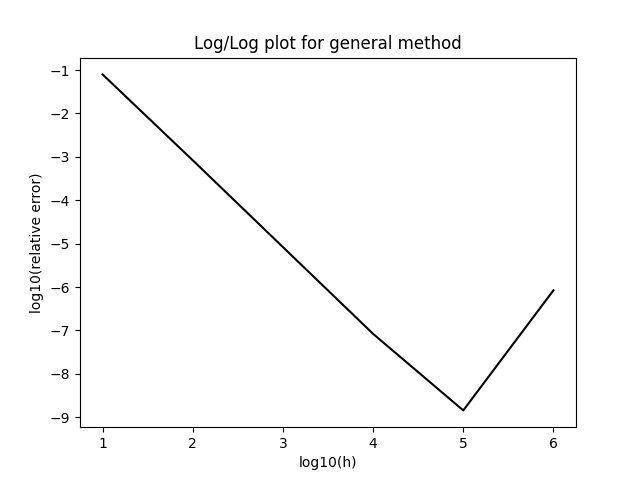
\includegraphics[width=0.9\linewidth]{../code/plots/error_general.png}
 \caption{The maximum deviation between the analytical solution and numerical solution for each $h$ for the general algorithm. This is presented as a log-log plot to account for the large differences in values. $h$ is the power of 10 for that spesific run.}
 \label{fig:errgeneral}
\end{subfigure}
\quad
\begin{subfigure}[b]{0.45\textwidth}
 \centering
 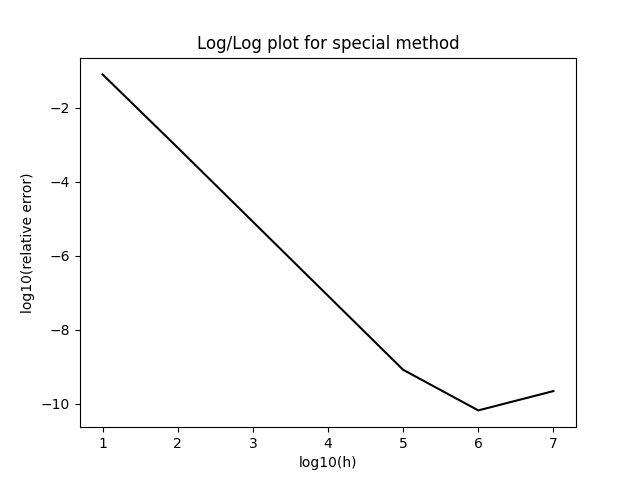
\includegraphics[width=0.9\linewidth]{../code/plots/error_special.png}
 \caption{The maximum deviation between the analytical solution and numerical solution for each $h$ for the specialzied algorithm. This is presented as a log-log plot to account for the large differences in values. $h$ is the power of 10 for that spesific run.}
 \label{fig:errspecial}
\end{subfigure}
\caption{Plots of the output data from the running of accompanying functions. Being general tridiagonal method and specialized tridiagonal method.}
\label{fig:fig}
\end{figure}

\begin{figure}
 \centering
 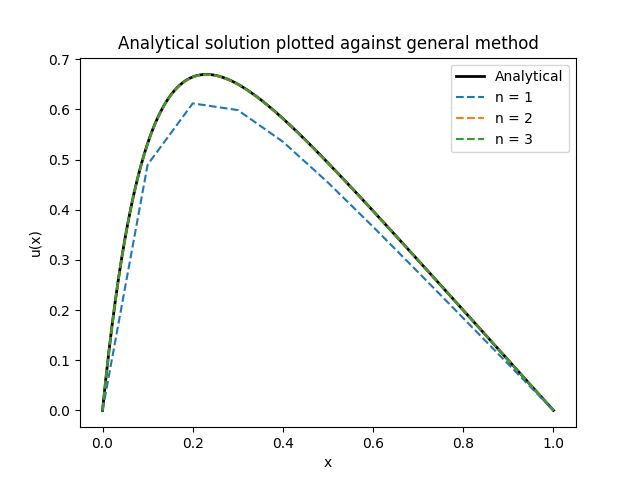
\includegraphics[width=0.9\linewidth]{../code/plots/plot_general.png}
 \caption{Plot of the specialized algorithm against the analytical solution. The plot shows runs for of the specialized algorithm with $h = 1, 2, 3$. End points are skipped in the plot for numerical solutions, as they do not affect the calculations and are set as $u(0) = u(n) = 0$.}
 \label{fig:general}
\end{figure}
\subsection{CPU time}
An important factor noted earlier was the difference in run time for the algorithms. In table \ref{tab:solver_times} it is clear that the relationship between runtimes is as expected. Data from Armadillo $solve()$ and lib.hpp functions are not included for $n>4$ as the tests where limited by memory. We clearly see that the relationship between the general and specialized algorithm is close to 1.5. Whilst for $solve()$ we can see that for $n=1$ that it performs significantly worse than for $n=2$. This could easily be to the analysis factor within the function. Including, running the normal LU decomposition for a 5x5 matrix, would not be sustainable. Performing an LU decomposition on a 4x4 matrix already takes around $\sim21$ minutes and increasing $n$ would result in another factor of $\sim$1000 increase in runtime. 
\begin{table}[h]
\caption{Table covering runtimes non-cold starts for all four algorithms used. Thoose being General, Specialized, Armadillos $solve$ and the library functions from lib.hpp. Data for Armadillo $solve$ and lib.hpp are not included for $n>4$ as it is limited by memory and could not be run in this test. All times are listed in seconds, unless spesified.}
\begin{tabular}{lcccc}
\hline
 $10^n$ & General & Specialized & $solve$ & lib.hpp \\ \hline
 1 & 0.00000024 & 0.00000021 & 0.00303977 & 0.00000318 \\
 2 & 0.00000164 & 0.00000140 & 0.00008639 & 0.00031194\\
 3 & 0.00001927 & 0.00001484 & 0.00644989 & 0.44017580\\
 4 & 0.00021870 & 0.00014394 & 0.58261636 & $\sim$21 minutes\\
 5 & 0.00223254 & 0.00147353 & n/a & n/a\\
 6 & 0.02110298 & 0.01508435 & n/a & n/a 
 \end{tabular}
\label{tab:solver_times}
\end{table}
\section{Discussion}
LU is a general algorithm , which works for all non-singular matricies and as such can be applied to almost any problem where $n$ is small. Our general algorithm takes a tridiagonal matrix and reduces it into a simpler algorithm which can handle a bigger $n$ at a much faster pace. Giving us a more efficent algorithm than for a dense matrix, where an entire $n$x$n$ matrix would need to be store, the general algorithm relies on three arrays of length $n$. 

As seen in talbe \ref{tab:solver_times} we can see that for the LU decomposition that for runtime the increase goes like $n$ cubed. Which makes it intolerable for larger $n$. On the same note, LU decomposition suffers from memory limitations, where memory needed goes like $n$ squared. For example for $h=5$ if we store the elements in our $n$x$n$ matrix $\mathbf{A}$ as doubles, we would need $8\times (10^5)^2 = 8 \times 10^10$ bytes on our computer. This is way more than any normal laptop or stationary computer have the ability to store, at $80$ giga bytes. If we where to need all three matrcies from an LU decomposition, namely A, L, U, we would need three times that amount to store all the matricies. This is way within reach that of a supercomputer\cite{OhioSupercomputerCenter1987}, however highly unnecessary when you have a tridiagonal matrix, or a matrix which can be solve with more efficient methods. 

This makes algorithm such as our general algorithm for a tridiagonal matrix and our specialized algorithm important parts of optimizing algorithms to be able to numerically solve problems at a fraction of the time, at a higher precision. This is apparent by looking at the number of FLOPs needed between especially LU and our specialized algorithm. However at the ability to run our program at lager values of $h$. Runtime wise we could go upto a very high value $n$ without reaching LU decomposition levels of runtime. However as seen in figure \ref{fig:general} we run into another problem with numerical analsys already at $n>10^5$. This is loss of numerical precision, due to the way computers store floating points numbers. Not all numbers can be represented exactly. For a double value in C++, we can store 64 bits of information, and this needs to store our entire number. Everything that does not fit, gets rounded off. The round off is very small, however when we perform FLOPs on the round off error quickly increase. If we perform a large amount of FLOPs on a number in one iteration, and keep doing so for the following, we can end up with an answer deviating far from our expected value. We can see a clear example of this in the difference between our general and specialized algorithm seen in figure \ref{fig:errgeneral} and \ref{fig:errspecial}. The specialized algorithm has roughly ($4n$)FLOPs and we can see that the algorithm suffers less from loss of numerically precision compared to the ($8n$)FLOPs for our general algorithm. 

The loss of numerical precision could also affect LU decomposition, as performing the decomposition goes like $\mathcal{O}(n^3)$FLOPs, however here we have a trade off between memory and numerical precision. If we take a look at the relationship between the runtime of the general algorithm and specialized algorithm, we would expect it to be of a factor 2. However not all FLOPs takes an equal amount of time, for small $n$ this is apparent. However as $n$ increases we should be able to see this relationship trending towards 2, at a loss of numerical precision, for $h>6$. 


\section{Conclusion}
As we have seen, the importance of developing efficient algorithms is essential to solving numerical problems. We have experienced the loss of numerical precision due to round off error and FLOPs. And looked at the ever increasing run time of general LU decomposition and memory limitations which comes with storing $n$x$n$ matricies in memory. 
We countered this by finding a discretized form of the second derivative and turning it into a linear algebra problem. Where we developed a general algorithm, which solved both the problem with memory and run time. With our specialized algorithm we were able to even further improve run time and reduced memory used. But we were still limited by numerical precision. 

Our specialized and general algorithm can be applied to most one dimensional second derivative problems with Dirichlet boundary conditions, and is a good way of solving such problems. Whilst LU decomposition still is the preffered choice for dense non-singular matricies, we also discorved that Armadillos $solve()$ is a good middle ground. The $solve()$ function proves to be a good choice, if the input matrix is not necessarily known, or developing an algorithm proves to be hard. Its runtime for dense non-singular matricies, is around the same as LU decomposition. 

Through brute force testing the specialized algorithm can possibly be improved, however the gain from doing so is marginal. The main limiter of this method is loss of numerical precision. For the remaining methods, all are as optimized as they can\cite{morten}. 
For the Armadillo\cite{Sanderson2016}\cite{DBLP:journals/corr/abs-1805-03380} library, we can only assume that the methods used are the most efficient ones known today. 

%\section{Theory}
%\subsection{The Poisson Equation}
%add section on poisson equation
%>> Dirilect boundary conditions >> relation between f(x) u'' >> Check equal
%\subsection{Approximation of the Second Derivative}
%Add section on approx of second derivative
%>> Going from diff equation >> linear form Av = b >> Matrix -1,2,-1
%\subsection{Relative Error}
%Add short theory of relative error
%>> YES


%%% footnote
% rainforest\footnote{Writing out a general case will also take up more paper
% space}.

%%% Matrix with line through between last elements
% \begin{equation}
% \left[
% \begin{array}{cccc|c}
% 1 & c_1/\beta_1 & 0 & 0 & \tilde{f}_1 \\
% 0 & 1 & c_2/\beta_2 & 0  & \tilde{f}_2 \\
% 0 & 0 & 1 & c_3/\beta_3 & \tilde{f}_3 \\
% 0 & 0 & 0 & 1 & \tilde{f}_4
% \end{array}
% \right] \sim
% \left[
% \begin{array}{cccc|c}
% 1 & c_1/\beta_1 & 0 & 0 & \tilde{f}_1 \\
% 0 & 1 & c_2/\beta_2 & 0  & \tilde{f}_2 \\
% 0 & 0 & 1 & 0 & \tilde{f}_3 -\frac{c_3}{\beta_3}\tilde{f}_4 \\
% 0 & 0 & 0 & 1 & \tilde{f}_4
% \end{array}
% \right]
% \end{equation}

%%% Listing
% \lstinputlisting[language=c++, firstline=146,
% lastline=158]{../problems.cpp}

%%% LU matrix, with diag dots for general case
% \begin{equation}
% A = LU =
% \begin{bmatrix}
% 1 & 0 & 0 & \dots & 0 & 0 \\
% l_{21} & 1 & 0 & \dots & 0 & 0 \\
% l_{31} & l_{32} & 1 & \dots & 0 & 0 \\
%   &\vdots & & \ddots & \vdots  & \\
% l_{n-11} & l_{n-12} & l_{n-13} & \dots & 1 & 0 \\
% l_{n1} & l_{n2} & l_{n3} & \dots & l_{nn-1} & 1
% \end{bmatrix}
% \begin{bmatrix}
% u_{11} & u_{12} & u_{13} & \dots & u_{1n-1} & u_{1n} \\
% 0 & u_{22} & u_{23} & \dots & u_{2n-1} & u_{2n} \\
% 0 & 0 & u_{33} & \dots & u_{3n-1} & u_{3n} \\
%   &\vdots & & \ddots & \vdots  & \\
% 0 & 0 & 0 & \dots & u_{n-1n-1} & u_{n-1n} \\
% 0 & 0 & 0 & \dots & 0 & u_{nn}
% \end{bmatrix}
% \end{equation}

%%% Table
% \begin{table}[h]
% \caption{Elapsed time for increasing $n$}
% \begin{tabular}{lcc}
% \hline
% n & TDMA [s] & LU [s] \\ \hline
% 10 & 0.0000035 & 0.00106083 \\
% 100 & 0.0000116 & 0.0022319 \\
% 1000 & 0.000077892 & 0.0677764 \\
% 10000 & 0.000878769 & 21.9247 \\
% 100000 & 0.00757418 & n/a \\
% 1000000 & 0.08616075 & n/a \\
% 10000000 & 0.76534 & n/a
% \end{tabular}
% \label{tab:solver_times}
% \end{table}

%%% Figure
% \begin{figure}[h]
  % \centering
  % \includegraphics[width=0.9\linewidth]{figures/relerror.png}
  % \caption{Plot of maximum relative error as a function of step size}
  % \label{fig:relerror}
% \end{figure}

%%% Cition and bilbliography%%
% # \emph{Thomas Algorithm} \cite{thomasalgo} How to cite.
% \begin{thebibliography}{10}
  % \bibitem{thomasalgo}{Thomas, L.H. (1949), \emph{Elliptic
        % Problems in Linear Differential Equations over a
        % Network}. Watson Sci. Comput. Lab Report, Columbia University,
      % New York.}
      % \bibitem{morten}{Hjorth-Jensen, M. (2015). \emph{Computational
        % Physics - Lecture Notes 2015}. University of Oslo}
    % \bibitem{golub}{Golub, G.H., van Loan, C.F. (1996). \emph{Matrix
          % Computations} (3rd ed.), Baltimore: John Hopkins.}
% \end{thebibliography}

\bibliography{bib_proj1}
\bibliographystyle{plain}


\end{document}
